\documentclass[tikz,border=10pt]{standalone}
\usepackage{tikz}
\usetikzlibrary{arrows.meta,positioning,calc,fit,backgrounds}

\definecolor{oanBlue}{HTML}{1F4E79}
\definecolor{oanTeal}{HTML}{0E7490}
\definecolor{oanGreen}{HTML}{2F855A}
\definecolor{oanGold}{HTML}{B7791F}
\definecolor{oanPurple}{HTML}{7C3AED}
\definecolor{oanSlate}{HTML}{334155}
\definecolor{oanCyan}{HTML}{155E75}
\definecolor{oanRose}{HTML}{9F1239}
\definecolor{oanGray}{HTML}{4A5568}
\definecolor{oanLight}{HTML}{F7FAFC}

\tikzset{
  layerbox/.style args={#1}{
    rounded corners=10pt,
    draw=#1!80,
    fill=#1!8,
    line width=1pt,
    inner xsep=7pt,
    inner ysep=4pt,
    align=center,
    font=\sffamily\tiny\bfseries
  },
  agentbox/.style args={#1}{
    rounded corners=9pt,
    draw=#1!80,
    fill=#1!10,
    line width=1pt,
    inner xsep=6pt,
    inner ysep=4pt,
    align=center,
    font=\sffamily\tiny\bfseries
  },
  regnode/.style={
    rounded corners=6pt,
    draw=oanGreen!85,
    fill=oanGreen!12,
    line width=0.9pt,
    inner xsep=6pt,
    inner ysep=4pt,
    font=\sffamily\tiny\bfseries,
    align=center
  },
  discnode/.style={
    rounded corners=6pt,
    draw=oanGold!85,
    fill=oanGold!12,
    line width=0.9pt,
    inner xsep=6pt,
    inner ysep=4pt,
    font=\sffamily\tiny\bfseries,
    align=center
  },
  vcnode/.style={
    rounded corners=6pt,
    draw=oanPurple!90,
    fill=oanPurple!8,
    line width=1pt,
    dash pattern=on 3.5pt off 1.8pt,
    inner xsep=6pt,
    inner ysep=4pt,
    font=\sffamily\tiny\bfseries,
    align=center
  },
  trust/.style={
    -{Latex[length=3mm,width=2mm]},
    line width=1pt,
    draw=oanBlue
  },
  publish/.style={
    -{Latex[length=3mm,width=2mm]},
    line width=1pt,
    draw=oanGreen
  },
  flow/.style={
    -{Latex[length=3mm,width=2mm]},
    line width=0.95pt,
    draw=oanGray
  },
  orbit/.style={
    draw=oanBlue!45,
    line width=0.95pt
  }
}

\begin{document}
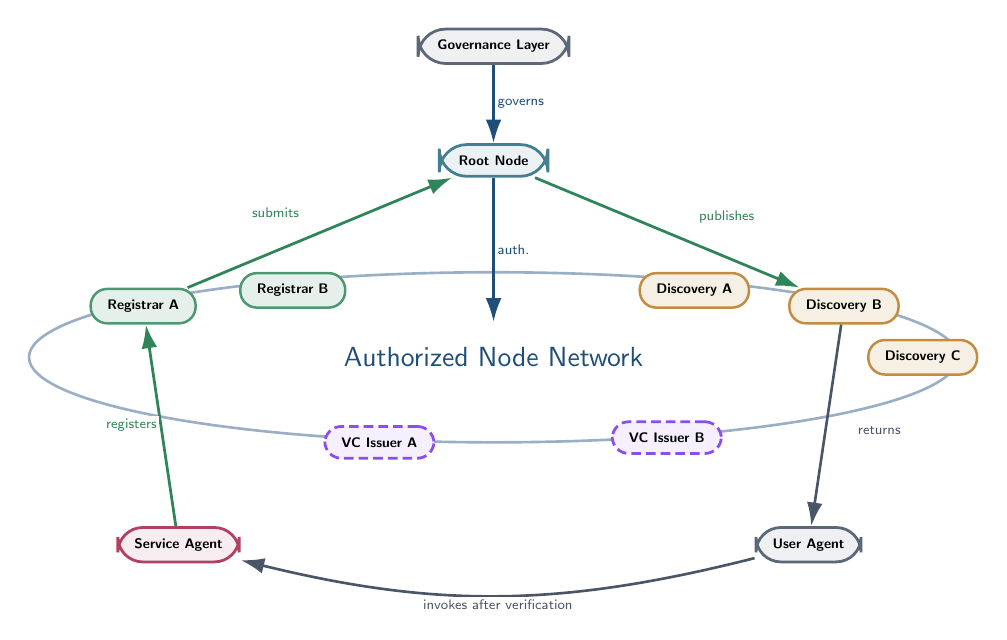
\begin{tikzpicture}[x=1cm,y=1cm]

\node[layerbox=oanSlate, draw=oanSlate!80, fill=oanSlate!8] (gov) at (0,5.65) {Governance Layer};
\node[layerbox=oanCyan, draw=oanCyan!80, fill=oanCyan!8] (root) at (0,4.2) {Root Node};

\draw[trust] (gov) -- node[right, font=\sffamily\tiny, text=oanBlue, fill=white, inner sep=1pt] {governs} (root);

\draw[orbit] (0,1.7) ellipse [x radius=5.9cm, y radius=1.08cm];
\node[font=\sffamily, text=oanBlue, fill=white, inner sep=1pt] at (0,1.7) {Authorized Node Network};

\node[regnode] (regA) at (-4.45,2.35) {Registrar A};
\node[regnode] (regB) at (-2.55,2.55) {Registrar B};

\node[discnode] (discA) at (2.55,2.55) {Discovery A};
\node[discnode] (discB) at (4.45,2.35) {Discovery B};
\node[discnode] (discC) at (5.45,1.7) {Discovery C};

\node[vcnode] (vcA) at (-1.45,0.62) {VC Issuer A};
\node[vcnode] (vcB) at (2.2,0.68) {VC Issuer B};

\node[agentbox=oanRose, draw=oanRose!80, fill=oanRose!8] (service) at (-4.0,-0.68) {Service Agent};
\node[agentbox=oanSlate, draw=oanSlate!80, fill=oanSlate!8] (user) at (4.0,-0.68) {User Agent};

\draw[trust] (root) -- node[right, font=\sffamily\tiny, text=oanBlue, fill=white, inner sep=1pt] {auth.} (0,2.15);

\draw[publish] (service) -- node[left, font=\sffamily\tiny, text=oanGreen, fill=white, inner sep=1pt] {registers} (regA);
\draw[publish] (regA) -- node[above left, font=\sffamily\tiny, text=oanGreen, fill=white, inner sep=1pt, xshift=-6pt, yshift=4pt] {submits} (root);

\draw[publish] (root) -- node[above right, font=\sffamily\tiny, text=oanGreen, fill=white, inner sep=1pt, xshift=10pt, yshift=2pt] {publishes} (discB);
\draw[flow] (discB) -- node[right, font=\sffamily\tiny, text=oanGray, fill=white, inner sep=1pt, xshift=10pt, yshift=-2pt] {returns} (user);
\draw[flow] (user) to[bend left=14] node[below, font=\sffamily\tiny, text=oanGray, fill=white, inner sep=1pt] {invokes after verification} (service);

\end{tikzpicture}
\end{document}
